
\begin{frame}

\begin{block}{Pattern matching}
Sélectionne une règle de réécriture à partir de la forme d'un terme.
\end{block}

\bigskip

\begin{block}{Types de pattern matching}
\begin{itemize}
\item Linéaire : \texttt{App(?x, ?y)}
\item Non linéaire : \texttt{App(?x, ?x)}
\end{itemize}
\end{block}

\end{frame}

\subsection{Pattern matching linéaire}

\begin{frame}
\frametitle{Exemple de pattern matching}

Soit le terme \texttt{Lambda(x, Var(x))}
\begin{itemize} 

  \item match \texttt{Lambda(\_, \_)}.
  \item mais pas \texttt{Var(\_)}.

\end{itemize}

\bigskip

\begin{block}{Extraction de sous-termes}
\texttt{Lambda(?x, \_)} retourne le sous-terme correspondant à \emph{?x}.
\end{block}

\end{frame}

\begin{frame}
\frametitle{Simulation}

Exemple du déroulement du pattern-matching:
\begin{itemize}
  
  \item Terme : \texttt{Lambda(y, Var(y))}.

  \item Pattern : \texttt{Lambda(\_, Var(?x))}.

\end{itemize}

\bigskip

\begin{center}
  \only<2>
      {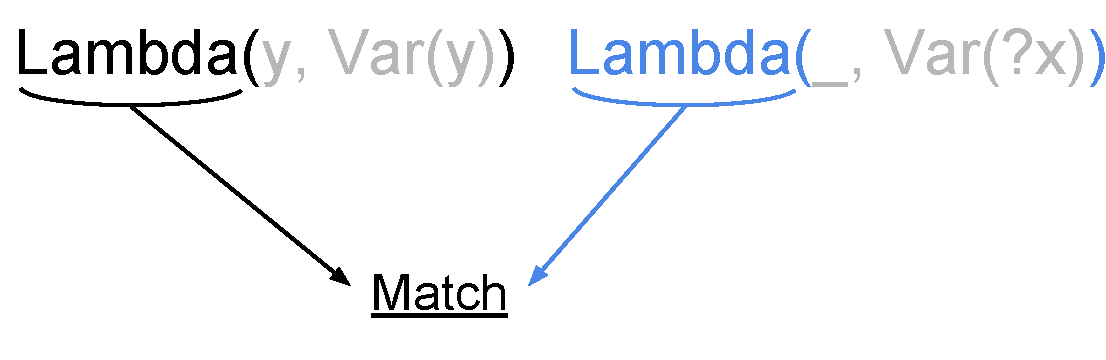
\includegraphics[scale=0.5]{pattern/trivial1.pdf}}
  \only<3>
      {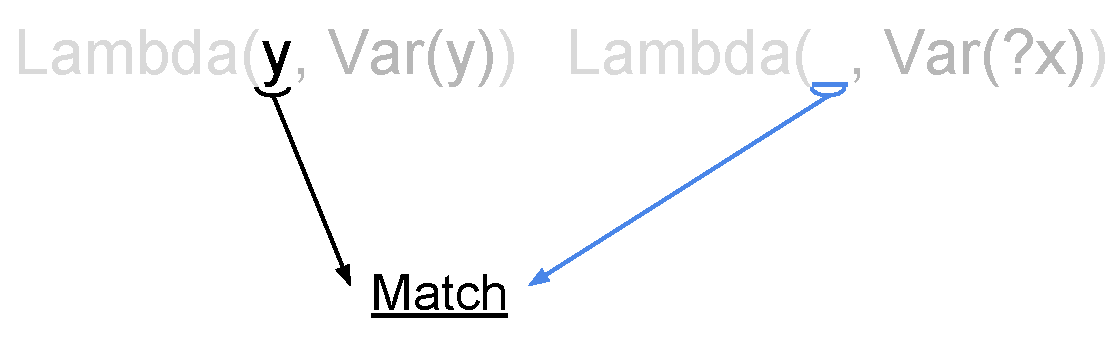
\includegraphics[scale=0.5]{pattern/trivial2.pdf}}
  \only<4>
      {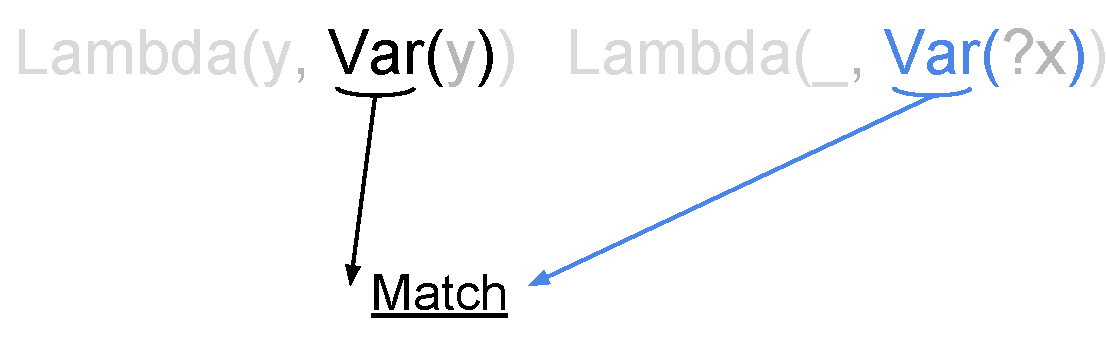
\includegraphics[scale=0.5]{pattern/trivial3.pdf}}
  \only<5>
      {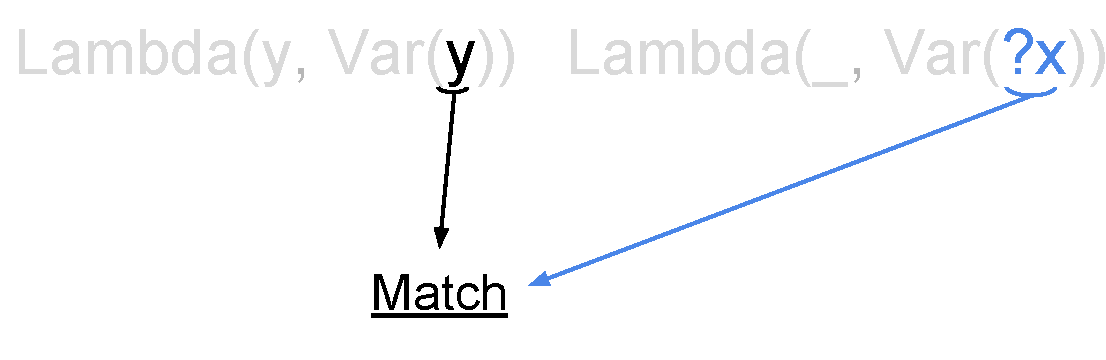
\includegraphics[scale=0.5]{pattern/trivial4.pdf}}
  \only<6>
      {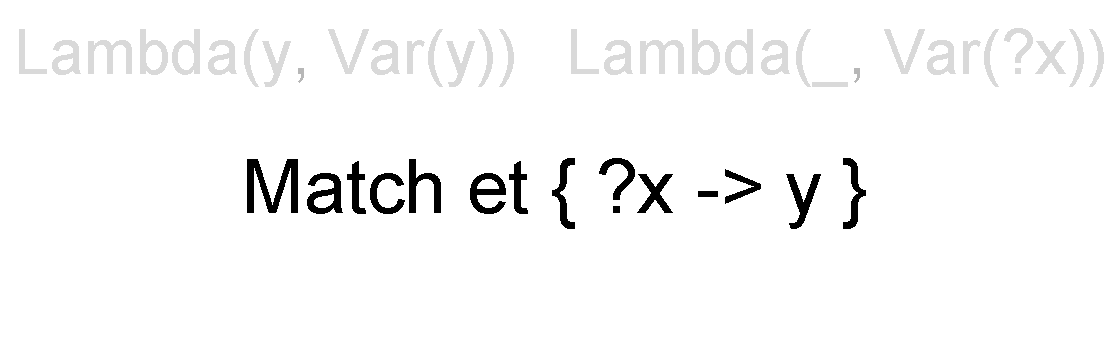
\includegraphics[scale=0.5]{pattern/trivial5.pdf}}

\end{center}

\end{frame}

\begin{frame}
\frametitle{Non linéarité des atomes}

Possibilité de matcher deux atomes liés même dans le cas linéaire.

Par exemple avec \texttt{Lambda(?x, Var(?x))} :

\bigskip
\begin{center}
  \only<2>
      {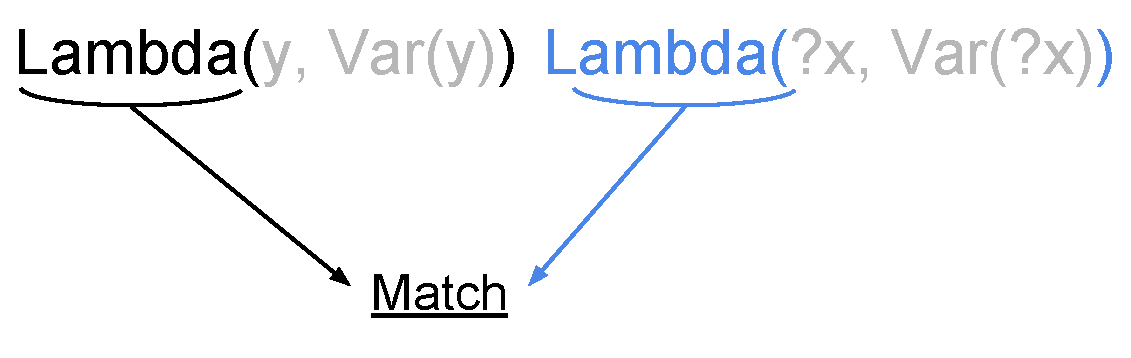
\includegraphics[scale=0.5]{pattern/atom1.pdf}}
  \only<3>
      {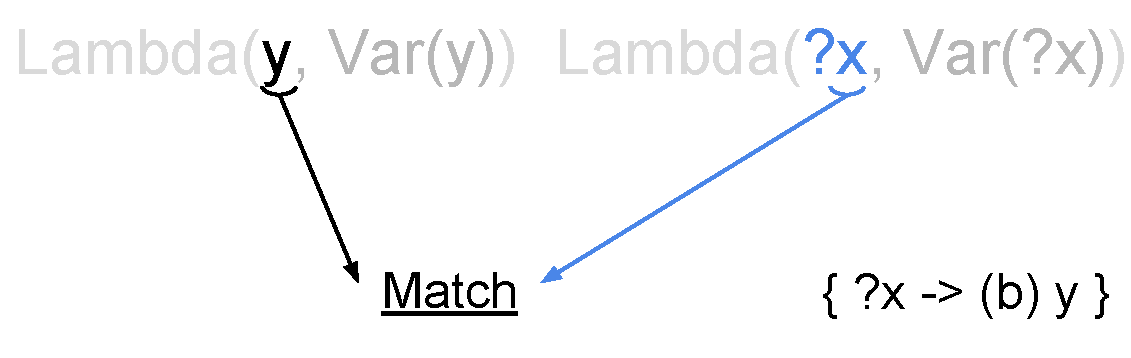
\includegraphics[scale=0.5]{pattern/atom2.pdf}}
  \only<4>
      {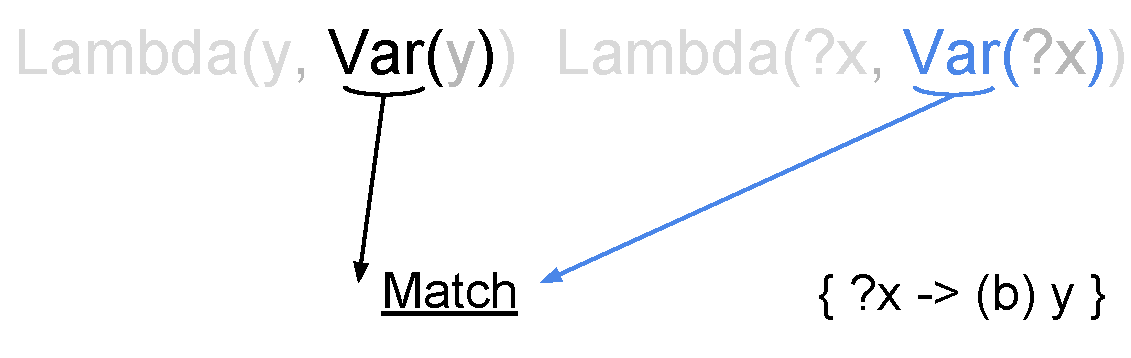
\includegraphics[scale=0.5]{pattern/atom3.pdf}}
  \only<5>
      {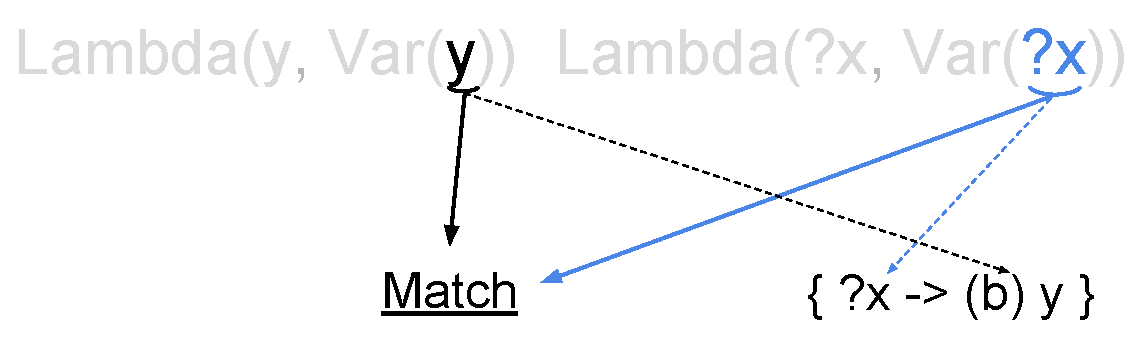
\includegraphics[scale=0.5]{pattern/atom4.pdf}}
  \only<6>
      {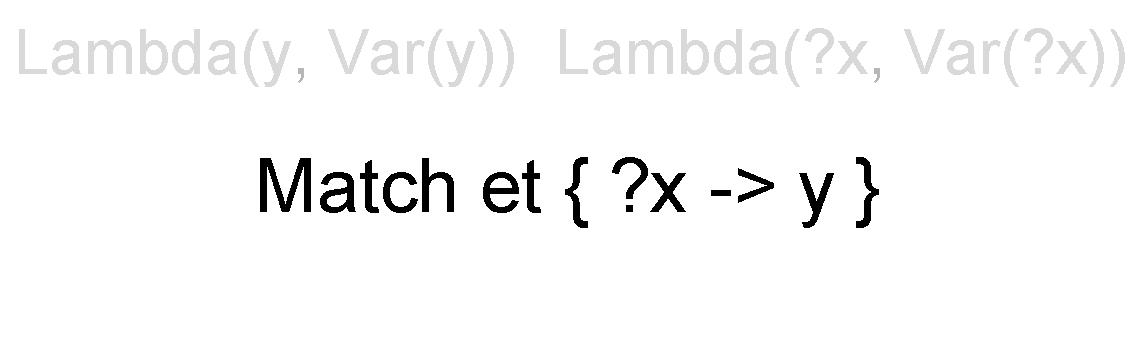
\includegraphics[scale=0.5]{pattern/atom5.pdf}}

\end{center}


\end{frame}

\subsection{Pattern matching non linéaire}

\begin{frame}
\frametitle{Non linéarité avec les termes}

\begin{block}{Non linéarité}
Possibilité d'extraire plusieurs fois le même motif modulo alpha-conversion.
\begin{itemize}
\item Atomes : possible dans l'algorithme linéaire.
\item Termes : nécessite la capacité de raisonner sur la structure du terme.
\end{itemize}
\end{block}

\pause

\begin{block}{Exemple}
\begin{itemize}
\item Terme : \texttt{App(Lambda(x, Var(x)), Lambda(y, Var(y)))} match
\item Pattern : \texttt{App(?X, ?X)}.
\end{itemize}
\end{block}

\medskip

Possible puisque le Lambda de droite n'est qu'un renommage du Lambda de gauche.

\end{frame}

\begin{frame}
\frametitle{Solution : hashconsing}

\begin{block}{Principe du hashconsing}
\begin{itemize}
\item Ne pas allouer deux fois deux structures identiques.
\item Deux termes structurellement identiques partagent l'allocation en mémoire.
\item Abstraction des noms de binders et de variables
liées.
\end{itemize}
\end{block}

\end{frame}

\begin{frame}[fragile]
\frametitle{Hashconsing : exemple d'égalité structurelle}

\begin{columns}
  \column{.5\textwidth}
  Pour le terme 
  \begin{verbatim}
  App(
     Lambda(x, Var(x)), 
     Lambda(y, Var(y))
  )
  \end{verbatim}

  \medskip

  \only<1>{
  
    \column{.5\textwidth}
    Avec hashconsing, l'équivalence structurelle apparait :
    \begin{center}
      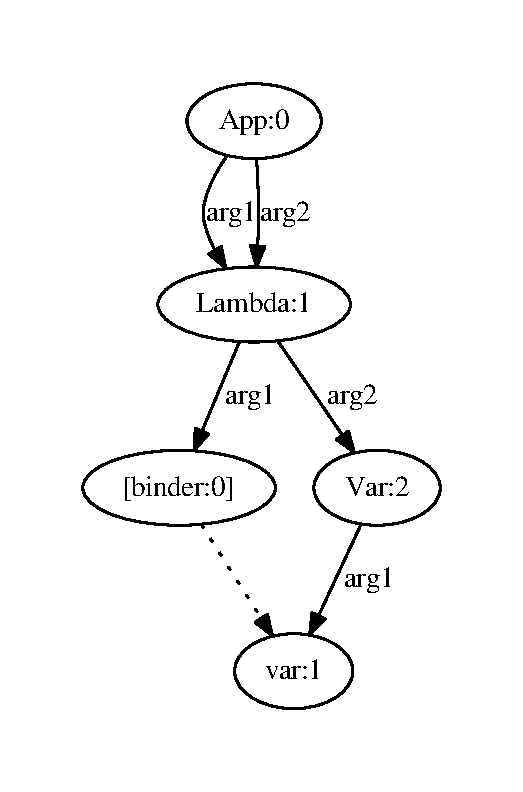
\includegraphics[scale=0.5]{pattern/pres_hash.pdf}
    \end{center}
  }
  
  \only<2>{
  
    \column{.5\textwidth}
    Sans hashconsing :
    \begin{center}
      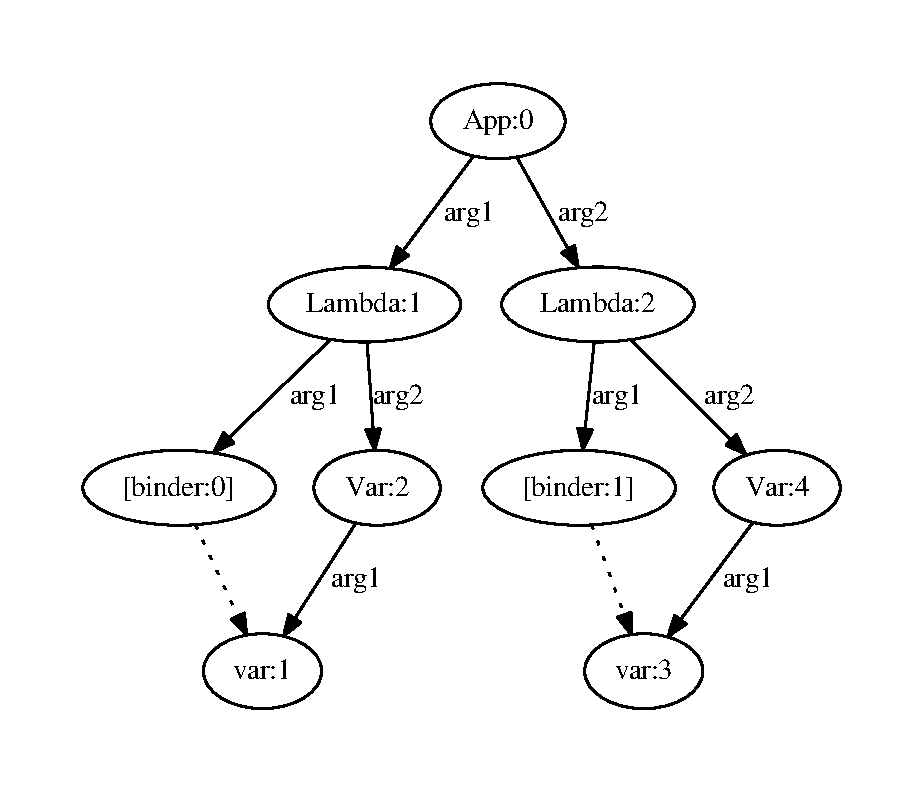
\includegraphics[scale=0.4]{pattern/no_hash.pdf}
    \end{center}
  }
\end{columns}
\end{frame}
